\section{Датчики IOT}
Самым важным оборудованием в IoT могут быть его датчики. Рисунок \ref{fig:section4:sensors} содержит примеры датчиков. Эти устройства могут считывать данные об электроэнергии, радиочастотные модули и сенсорные модули. ВЧ-модули управляют связи через их обработку сигналов, WiFi, ZigBee, Bluetooth, RF.

\begin{figure}[h!]
    \centering
    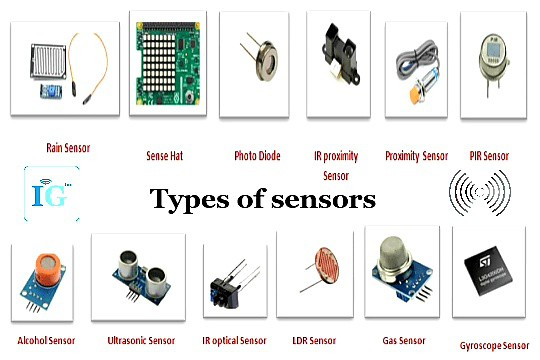
\includegraphics[scale=0.7]{sensors.png}
    \caption{Датчики IOT}
    \label{fig:section4:sensors}
\end{figure}

Сенсорный модуль управляет считыванием с помощью различных активных и пассивных элементов.
устройства. Вот список некоторых датчиков, используемых в IoT:
\begin{itemize}
    \item акселерометры
    \item магнитометры
    \item гироскопы
    \item акустические датчики
    \item датчики давления, газа, влажности, света
    \item RFID
\end{itemize}

\subsection{Носимая электроника}
Носимые электронные устройства — это небольшие устройства, которые носят на голове, шее, руках, туловище и ступнях.
Умные часы не только помогают нам оставаться на связи и отслеживают нашу физическую активность, но и являются частью Интернета вещей.\cite{IoTArch}
Умные носимые устройства включают в себя:
\begin{itemize}
    \item Голова – Шлемы, очки
    \item Шея – украшения, воротники
    \item Рука – Часы, браслеты, кольца
    \item Торс – Одежда, рюкзаки
    \item Ноги – носки, обувь
\end{itemize}

\subsection{Стандартные устройства}
Компьютер, ноутбук, планшет и мобильный телефон остаются неотъемлемыми частями Интернета вещей в качестве \\командного центра и
элементом управления системой.
\begin{itemize}
    \item Компьютер предоставляет пользователю наивысший уровень контроля над системой и ее
    настройками.
    \item Планшет обеспечивает доступ к ключевым функциям системы способом, напоминающим
    рабочий стол, а также выступает в роли элемента управления.
    \item Мобильный телефон позволяет изменять некоторые важные настройки, а также обеспечивает дистанционное управление функциональностью.
\end{itemize}
Другие ключевые подключенные устройства включают стандартные сетевые устройства, такие как маршрутизаторы и коммутаторы.